\chapter{树、路径与有根树基础}
\label{chap:trees}

\section*{本章目标}
本章系统介绍图、树、路径、有根树和最近公共祖先等概念，并把它们翻译成配电网语言。读完本章后，应能判断一个隐藏分支节点是否具有可辨识意义，并理解\cref{chap:mst}中 MST 算法为什么能利用割和环的结构。

\section{图、路径、连通性与无环性}

\begin{definition}[无向图]
无向图 $G=(V,E)$ 由有限节点集 $V$ 和无向边集 $E\subseteq \{\{i,j\}:i,j\in V,i\ne j\}$ 构成。若 $e=\{i,j\}\in E$，称 $i$ 与 $j$ 相邻。
\end{definition}

\begin{definition}[路径和简单路径]
从 $v_0$ 到 $v_k$ 的路径是节点序列 $(v_0,v_1,\ldots,v_k)$，满足 $\{v_{\ell-1},v_\ell\}\in E$。若路径中节点互不重复，则称为简单路径。路径长度可以指边数，也可以指边权和；本书会根据上下文说明。
\end{definition}

\begin{definition}[连通与环]
若任意两个节点之间均存在路径，则图连通。若存在 $k\ge 3$ 且 $v_0=v_k$、$v_0,\ldots,v_{k-1}$ 互异的路径，则称图含环。
\end{definition}

\begin{theorem}[树的等价刻画]
\label{thm:tree_equiv}
对有限无向图 $T=(V,E)$，以下命题等价：
\begin{enumerate}[label=(\roman*)]
  \item $T$ 连通且无环；
  \item 任意两个节点之间存在唯一简单路径；
  \item $T$ 连通且 $|E|=|V|-1$；
  \item $T$ 无环且 $|E|=|V|-1$。
\end{enumerate}
\end{theorem}

\begin{proof}
若 $T$ 连通且无环，则任意两点至少有一条路径；若有两条不同简单路径，它们合并会形成环，矛盾，所以路径唯一。若任意两点有唯一简单路径，则图连通；若有环，环上两点之间有两条不同路径，矛盾，所以无环。连通无环图从一个节点开始逐步加入新节点，每加入一个节点必须且只需一条连接到已有部分的边，因此有 $|E|=|V|-1$。反过来，连通图若含环，删去环上一条边仍连通，会得到边数至少 $|V|$ 的冗余结构；无环图若不连通，则每个连通分量都是树，边数为 $\sum_r(|V_r|-1)=|V|-c<|V|-1$。于是得到等价性。
\end{proof}

\section{有根树、父子关系与深度}

指定根节点 $0$ 后，树中任意节点 $i$ 到根有唯一路径，记为
\begin{equation}
  \pathset_{0i}=(0=v_0,v_1,\ldots,v_k=i).
\end{equation}
节点 $i$ 的深度定义为 $\operatorname{depth}(i)=k$。若边带正权 $w_e$，也可定义加权深度
\begin{equation}
  h(i)=\sum_{e\in \pathset_{0i}} w_e .
\end{equation}
配电网中，深度常对应离电源的电气距离或线路层级；加权深度可对应公共路径阻抗和。

\begin{definition}[最近公共祖先]
在有根树中，节点 $i,j$ 的最近公共祖先 $\lca(i,j)$ 是同时位于 $\pathset_{0i}$ 与 $\pathset_{0j}$ 上、且深度最大的节点。
\end{definition}

\begin{proposition}[树上距离的 LCA 表达]
\label{prop:lca_distance}
若每条边权 $w_e>0$，令 $h(i)$ 为根到 $i$ 的加权深度，则
\begin{equation}
  d_T(i,j)=h(i)+h(j)-2h(\lca(i,j)).
\end{equation}
\end{proposition}

\begin{proof}
从 $i$ 到 $j$ 的唯一路径由 $i$ 上行到 $\lca(i,j)$，再下行到 $j$。第一段权重为 $h(i)-h(\lca(i,j))$，第二段为 $h(j)-h(\lca(i,j))$，相加即得结论。
\end{proof}

\section{配电网中的隐藏分支节点}

\begin{figure}[htbp]
  \centering
  \begin{tikzpicture}[
  node distance=1.35cm and 1.45cm,
  every node/.style={font=\small},
  obs/.style={circle,draw,fill=blue!18,minimum size=7mm},
  hid/.style={circle,draw,fill=white,minimum size=7mm},
  root/.style={circle,draw,fill=black!12,minimum size=7mm},
  line/.style={-Latex,thick}
]
\node[root] (r) {$0$};
\node[hid,below=of r] (a) {$a$};
\node[obs,below left=of a] (n1) {$1$};
\node[obs,below=of a] (n2) {$2$};
\node[hid,below right=of a] (b) {$b$};
\node[obs,below left=of b] (n3) {$3$};
\node[obs,below right=of b] (n4) {$4$};
\draw[thick] (r)--(a)--(n1);
\draw[thick] (a)--(n2);
\draw[thick] (a)--(b)--(n3);
\draw[thick] (b)--(n4);
\node[align=center,right=1.0cm of b] {隐藏分支点\\未直接量测};
\end{tikzpicture}

  \caption{配电网有根树与隐藏分支节点示意。实心节点表示可观测电表，空心节点表示未量测分支点。}
  \label{fig:distribution_tree_hidden}
\end{figure}

\Cref{fig:distribution_tree_hidden}展示了一个典型场景。根节点 $0$ 是台区总表，$a,b$ 是隐藏分支点，$1,2,3,4$ 是用户表。量测矩阵只包含用户侧曲线时，算法必须从叶节点间距离中恢复 $a,b$ 的存在。

\section{度为 2 隐藏节点为何不可唯一恢复}

\begin{definition}[度为 2 隐藏节点压缩]
若隐藏节点 $h$ 的度为 $2$，相邻边为 $(u,h)$ 与 $(h,v)$，且边权为 $w_{uh},w_{hv}$，则可把两条边压缩成一条边 $(u,v)$，权重为 $w_{uh}+w_{hv}$。压缩后所有可观测节点间的路径距离保持不变。
\end{definition}

\begin{proposition}[度为 2 隐藏节点不可由叶间距离唯一辨识]
\label{prop:degree2_unidentifiable}
若只观测某个集合 $L$ 上的两两路径距离，则任意不属于 $L$ 的度为 $2$ 隐藏节点及其相邻两条边的拆分比例不可唯一恢复。
\end{proposition}

\begin{proof}
设隐藏节点 $h$ 只连接 $u$ 与 $v$。对任意两个可观测节点 $i,j\in L$，若路径不经过 $h$，距离不变；若路径经过 $h$，贡献总是 $w_{uh}+w_{hv}$。把 $w_{uh},w_{hv}$ 替换为任意正数 $\alpha,\beta$ 且 $\alpha+\beta=w_{uh}+w_{hv}$，所有 $d(i,j)$ 完全相同。因此叶间距离不能识别 $h$ 的位置或两段边权。
\end{proof}

\begin{figure}[htbp]
  \centering
  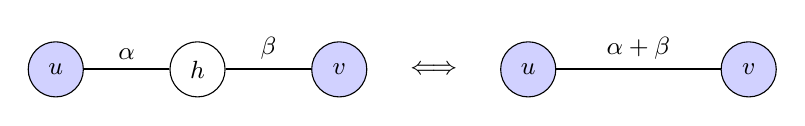
\begin{tikzpicture}[
  every node/.style={font=\small},
  obs/.style={circle,draw,fill=blue!18,minimum size=7mm},
  hid/.style={circle,draw,fill=white,minimum size=7mm}
]
\node[obs] (u) at (0,0) {$u$};
\node[hid] (h) at (1.8,0) {$h$};
\node[obs] (v) at (3.6,0) {$v$};
\draw[thick] (u)--node[above] {$\alpha$} (h)--node[above] {$\beta$} (v);
\node at (4.8,0) {$\Longleftrightarrow$};
\node[obs] (u2) at (6.0,0) {$u$};
\node[obs] (v2) at (8.8,0) {$v$};
\draw[thick] (u2)--node[above] {$\alpha+\beta$} (v2);
\end{tikzpicture}

  \caption{度为 $2$ 隐藏节点压缩前后对端点距离等价。}
  \label{fig:degree2_hidden}
\end{figure}

\begin{example}[线路中点是否为节点]
若一条从分支箱到用户的电缆中间有一个未装表接头，且该接头不产生新的支路，则从拓扑辨识角度它是度为 $2$ 隐藏节点。仅靠端点电压功率曲线，不能判断这条线路是“一段”还是“两段”，只能估计总阻抗。
\end{example}

\section{本章小结}

树的关键特征是任意两点间路径唯一，这使路径距离、LCA 和公共路径阻抗都有明确含义。有根树把电源端方向引入图模型，便于解释父节点、子节点和分支层级。隐藏节点若度至少为 $3$，可能从叶间距离中体现为多个叶节点簇共享分支；若度为 $2$，则只能恢复压缩后的等效拓扑。这一事实解释了为什么\cref{chap:hidden_tree}讨论的隐藏树重构通常默认隐藏节点度至少为 $3$。

\section*{思考题}
\begin{enumerate}
  \item 证明：树中任意一条边都是割边，即删除它会使图不连通。
  \item 对\cref{fig:distribution_tree_hidden}，写出 $\lca(1,2)$、$\lca(1,4)$ 与 $\lca(3,4)$。
  \item 若一个隐藏节点度为 $4$，它是否一定可由叶间距离稳定恢复？还需要哪些条件？
  \item 解释为什么线路接头、熔断器、分支箱在不同数据粒度下可能对应不同的图节点定义。
\end{enumerate}
